Der Naschmarkt ist mithilfe des open source Web Application Frameworks Laravel\cite{laravel} entwickelt.
Dieses folgt dem MVC-Muster.
Daher k\"onnen auch in der Klassenstruktur die Komponenten dieses Musters (Models und Controller) erkannt werden.
Es folgt das UML-Klassendiagramm der Applikation.
Rot dargestellt sind dabei die Komponenten des Frameworks, Gelb die Klassen und Interfaces der Applikation.

\begin{sidewaysfigure}
    \begin{center}
		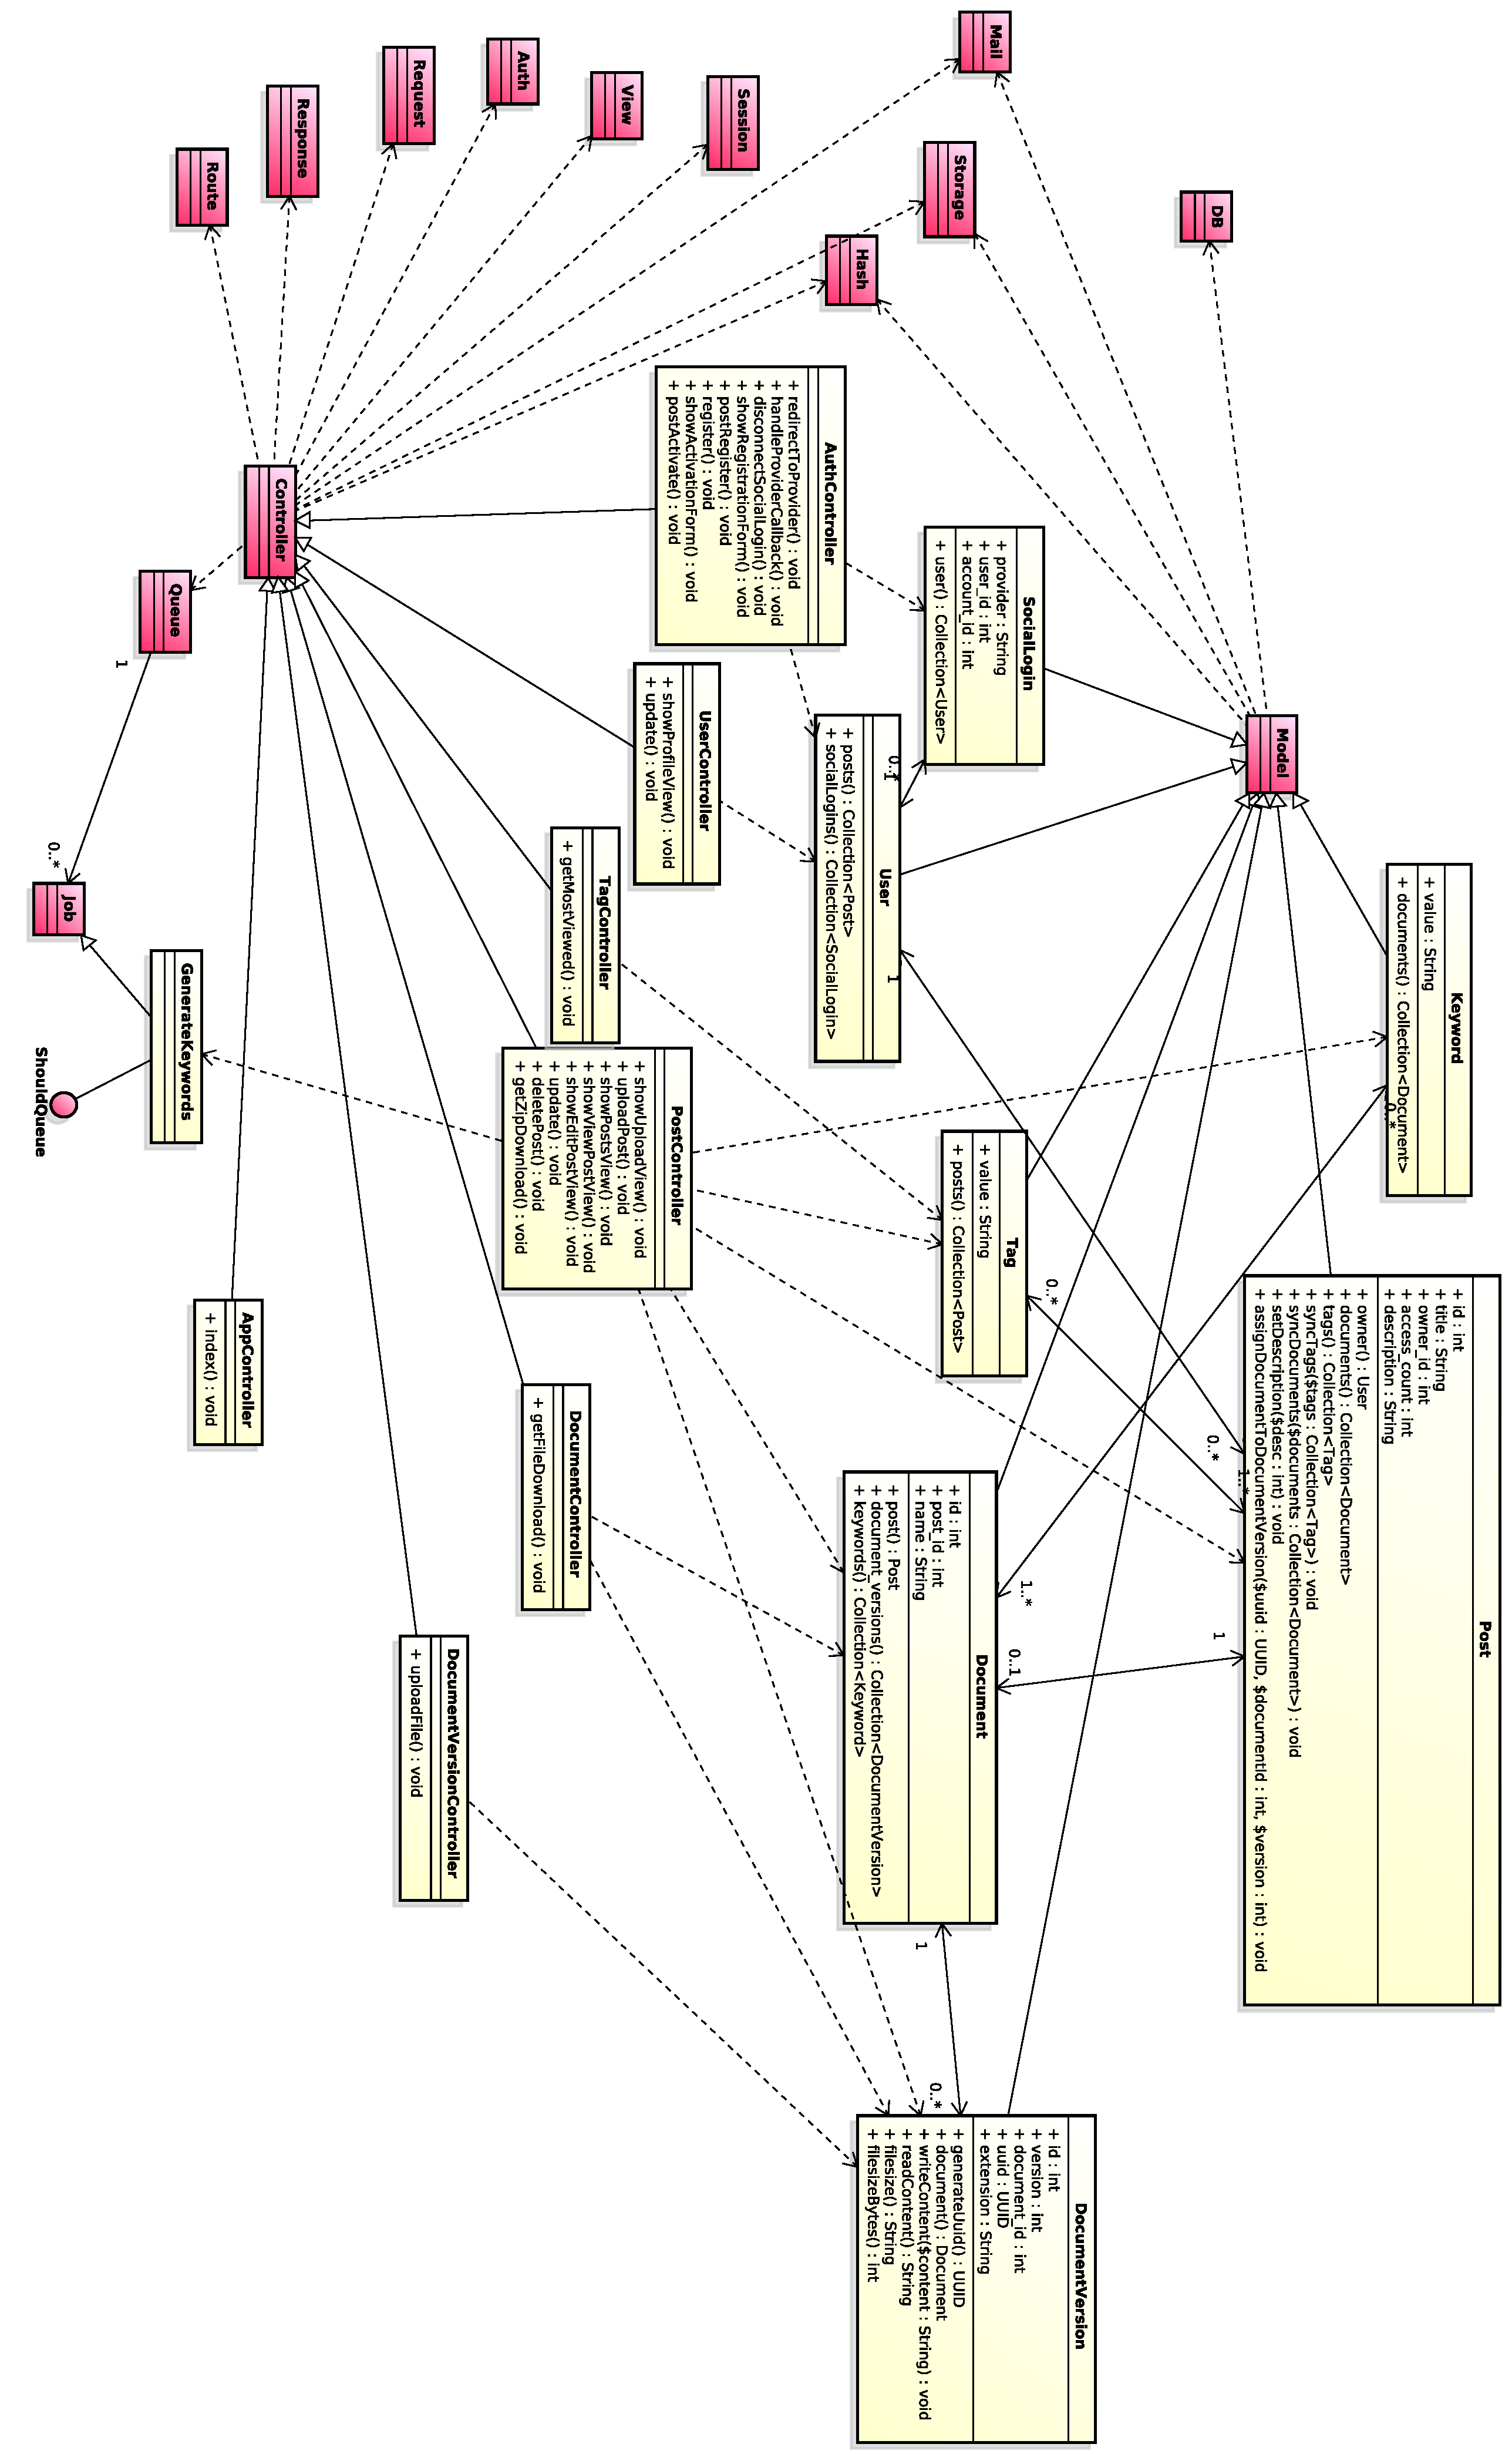
\includegraphics[width=\linewidth]{images/UML_Classdiagramm.pdf}
		\caption{UML Diagramm}
    \end{center}
\end{sidewaysfigure}

\clearpage
\section{Use Case Diagramm}
Folgendes Use Case Diagram zeigt die Anwendungsf\"alle des Naschmarktes.

\begin{figure}[H]
	\begin{center}
		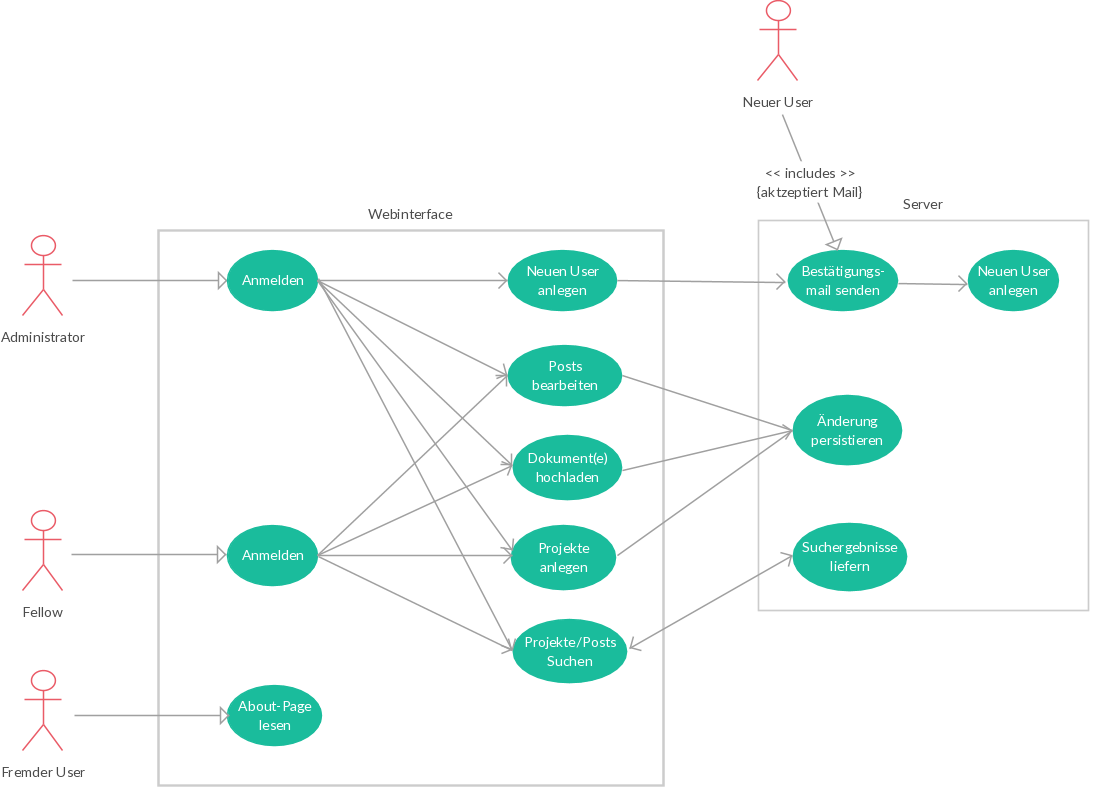
\includegraphics[width=\linewidth]{images/use_case.png}
		\caption{Use Case Diagramm}
	\end{center}
\end{figure}
